\documentclass[ppgc,pep]{iiufrgs}

% Use unicode
\usepackage[utf8]{inputenc}   % pacote para acentuação

% Necessário para incluir figuras
\usepackage{graphicx}           % pacote para importar figuras

\usepackage{times}              % pacote para usar fonte Adobe Times
% \usepackage{palatino}
% \usepackage{mathptmx}          % p/ usar fonte Adobe Times nas fórmulas

\usepackage[alf,abnt-emphasize=bf]{abntex2cite}	% pacote para usar citações abnt

\title{Mineração de dados de GPS para descoberta de padrões de mobilidade}
\author{Zembrzuski}{Rodrigo Claro}
\advisor[Prof.~Dr.]{Barone}{Dante Augusto Couto}
% a data deve ser a da defesa; se nao especificada, são gerados
% mes e ano correntes
\date{Outubro}{2017}
\location{Porto Alegre}{RS}

\keyword{análise de dados}
\keyword{análise espaçotemporal}
\keyword{aprendizado de máquina}
\keyword{padrões periódicos}
\keyword{padrões de mobilidade}
\keyword{computação móvel}
\keyword{mineração de dados}
\keyword{GPS}

\begin{document}

% folha de rosto
% às vezes é necessário redefinir algum comando logo antes de produzir
% a folha de rosto:
% \renewcommand{\coordname}{Coordenadora do Curso}
\makeatletter
\let\@makenominatapage\relax
\makeatother
\maketitle

\begin{abstract}
Com a presença massiva de equipamentos de GPS, presentes na maioria dos smartphones, o comportamento 
de mobilidade de muitos indivíduos vem sendo constantemente capturado. Este trabalho 
se propõe a aplicar técnicas de mineração de dados para obtenção de padrões de mobilidade em 
bancos de dados alimentados por GPS. Esses padrões poderão ser utilizados para predizer futuros
locais significativos, descoberta de rotas comuns e descoberta de atividades baseadas no local
em que uma determinada pessoa frequenta.
\end{abstract}

\chapter{Introdução}

A mineração de padrões de mobilidade de indivíduos é uma
área de pesquisa emergente. O gerenciamento eficiente
de dados espaçotemporais vem ganhando muito interesse nos
últimos anos [B14, B16, B6, B15], principalmente devido
ao rápido avanço das telecomunicações (GPSs, dados de
celular, etc.), que facilitam a coleta de grandes {\it datasets}
com essas informações. O gerenciamento e análise de trajetórias
é muito desafiador, dada a vasta quantidade de dados
coletados e novos tipos de consultas espaçotemporais.

Apesar das grandes dissimilaridades nas distâncias percorridas
pelos indivíduos, desde alguns quilômetros até centenas
de quilômetros, a mobilidade dos indivíduos mostra-se altamente
regular [1]. Em muitos casos, os movimentos obedecem padrões
periódicos, isto é, seguem aproximadamente as mesmas rotas
sob intervalos de tempo regulares. Por exemplo, João acorda
mais ou menos no mesmo horário todo dia, vai ao trabalho
pelo mesmo local todos os dias. Além disso, muitos indivíduos 
retornam aos mesmos lugares e
possuem a mesma função de densidade de probabilidade para
os lugares visitados [2]. Após a remoção de outliers, as regras
que determinam a exploração de novas localizações ou retorno a 
lugares já visitados parecem ser muito similares [3]. Além disso,
membros do mesmo grupo social, como pesquisadores do mesmo 
laboratŕoio, apresentam comportamentos semelhantes [4].

Mesmo assim, o problema da descoberta de padrões periódicos a partir de
dados históricos é muito desafiador. Frequentemente, os padrões
não são tão explícitos, mas podem ser inferidos com os dados. Os
padrões podem ser vistos como uma sequencia de localizações que 
reaparecem no histórico de movimentação de um indivíduo periodicamente.
Um grande desafio é que não se espera que o mesmo indívduo esteja
exatamente no mesmo lugar no mesmo instante a cada período. Os
padrões não são rígidos, mas se diferenciam levemente de uma
ocorrência parra outra. Essa natureza aproximada -- e não exata --
no domínio de dados espaçotemporais aumenta enormemente a complexidade
da tarefa de mineração.


%\section{Abordagens em mineração das trajetŕórias}

%São apresetnta duas abordagens para descrever os padrões das trajetórias. Na primeira abordagem,
%as trajetórias são descritas como transições entre locais de significância para cada
%cenário. Desse modo, a mobilidade de um indivíduo é descrito como um grafo, em que
%cada nodo indica os locais pelo qual o indivíduo passou e as edges são enriquecidas com
%outras features, como a duração das transições e suas frequencias. FULANO faz um trabalho
%muito sólido com essa abordagem, que XXXX. 

%No segundo tipo de abordagem, as trajetórias são convertidos para itens espaçotemporais, em
%que cada padrão periódico é descoberto. BELTRANO faz um trabalho muito sólido com essa 
%abordagem, que XXXXX.

%Vou citar o trabalho mais relevante dos grafos.

%Vou citar o trabalho mais relevante do spatio-temporal.


\section{Definição do problema}


\begin{figure}[h]
	\centering
	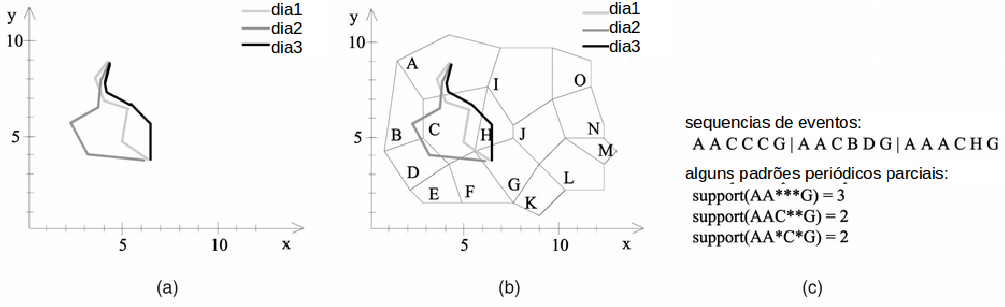
\includegraphics[width=1\textwidth]{figurinha2}
	\caption{Padrões periódicos com respeito a regiões espaciais predefinidas. (a) Movimento do objeto (b) Um conjunto
	de regiões predefinidas. (c) Padrões baseados em eventos.}
	\label{crisp-dm}
\end{figure}


%The problem of mining sequential patterns from transac-
%tional databases has attracted a lot of interest since Agrawal
%and Srikant introduced it in [2]. Each transaction contains a
%set of items that are bought by some customer, and the
%database consists of ordered lists of transactions. For
%example, hða; bÞ; ða; cÞ; ðbÞi is a sequence containing three
%transactions ða; bÞ, ða; cÞ, and ðbÞ. Given such a database, the
%sequential pattern mining problem is to find ordered lists of
%itemsets that appear in sequences with high frequency. For
%instance, hðbÞ; ðaÞ; ðbÞi is a pattern which is supported by the
%above sequence. The original sequential pattern mining
%problem does not consider the periodicity character of a
%transaction sequence.

%Periodicity has only been studied in the context of time-
%series databases. Indyk et al. [9] address the following
%problem: Given a long sequence S and a period T , the aim is
%to discover the most representative trend that repeats itself
%in S every T timestamps. Exact search might be slow; thus,
%[9] proposes an approximate technique based on sketches.
%However, the discovered trend for a given T is only one and
%spans the whole periodic interval. In [12], the problem of
%finding association rules that repeat themselves in every
%period of a data sequence is addressed. Elfeky et al. in [4]
%tackle the problem of periodicity detection on a series of
%nominal data, focusing on the automatic detection of the
%period.


HUIPING CAO define o problema da mineração de padrões
periódicos em dados espaçotemporais. No modelo proposto,
assume-se que as localizações são amostradas por um histórico
longo. Em outras palavras, o movimento de um objeto é capturado
como uma sequência de tamanho n. Essa sequencia possui 
as coordenadas e seu respectivo {\it timestamp} na seguinte forma:


\begin{equation}
\{(l_0, t_0), (l_1, t_1), ..., (l_{n-1}, t_{n-1})\}
\end{equation}

Na equação (1.1), {\it l\textsubscript{i}} é a localização do objeto no tempo {\it t\textsubscript{i}}.
Se a diferença entre os {\it timestamps} consecutivos é fixa -- isto é,
se as localizações são amostravadas em intervalos de tempo regulares --,
podemos representar o movimento por uma sequencia simples de localizações
{\it l\textsubscript{i}}, ou seja, sem os timestamps {\it t\textsubscript{i}}, uma vez que eles podem ser inferidos.

Cada localização {\it l\textsubscript{i}} é expressa em termos de coordenadas espaciais. 
 Fig. 1.1, por exemplo, ilustra
o movimento de um objeto em três dias consecutivos
(assumindo que eles são registrados em horários repetidos). 
Pode-se modelá-los com a sequencia definida em (1.2). 

\begin{equation}
S = \{ \langle 4, 9 \rangle, \langle 3.5, 8 \rangle, ..., \langle 6.5, 3.9 \rangle, \langle 4.1, 9 \rangle, ... \}
\end{equation}


Dada essa sequencia, um suporte minimo {\it min\_sup} (0 < {\it min\_sup} <1) e um inteiro {\it T}, chamado
período, o problema é descobrir padrões de movimentos que se repetem
a cada T {\it timestamps}. 



\chapter{Objetivos}

O principal objetivo do trabalho é o estudo e avaliação das principais
técnicas encontradas no meio acadêmico para predição de padrões periódicos
de mobilidade.

Será criado um {\it dataset} com 30\% da base de dados Geolife [X],
que contém dados de geolocalização. Este dataset será para uso exclusivo
em {\it benchmarks} para comparação de performance das soluções propostas.

Serão avaliadas possíveis métricas para avaliação dos algoritmos propostos 
e escolhida a mais adequada. Também serão avaliadas técnicas de clusterização 
de trajetórias, técnicas baseadas em grafos e técnias baseadas em trajetórias 
espaçotemporais. 

Baseado no estudo feito, poderá ser proposta, ainda, uma técnica que misture duas ou
mais abordagens já propostas na literatura.



\chapter{Metodologia}

Este trabalho seguirá a tradicional metodologia CRISP-DM para projetos de ciência de dados. Tal metodologia consiste em um processo cíclico composto por seis etapas (AZEVEDO; SANTOS, 2008):

\begin{figure}[h]
	\caption{Fluxograma da metodologia CRISP-DM}
	\centering
	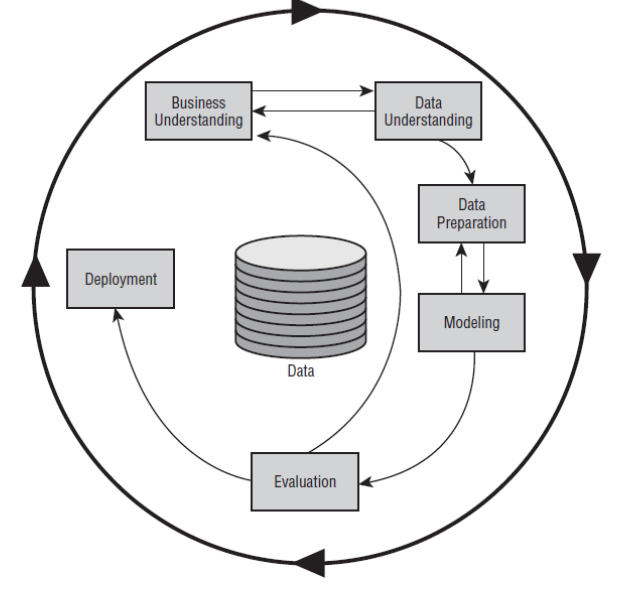
\includegraphics[width=0.75\textwidth]{crispdm}
	\label{crisp-dm}
\end{figure}

\begin{enumerate}
	\item \textbf{Compreensão do negócio} - Consiste em compreender os requisitos e objetivos do projeto e convertê-lo em um problema de mineração de dados, elaborando também um plano inicial para atingir seus objetivos.
	\item \textbf{Compreensão de dados} - Coleta e análise exploratória dos dados, para descoberta de eventuais problemas nos mesmos e detecção de padrões interessantes para geração de hipóteses.
	\item \textbf{Preparação de dados} - Atividades relacionadas ao refinamento dos dados brutos para construção da base de dados final a ser utilizada.
	\item \textbf{Modelagem} - Criação de modelos sobre os dados e calibração para otimizar seus parâmetros. No contexto deste trabalho, envolve o uso de técnicas de aprendizado de máquina.
	\item \textbf{Avaliação} - Os modelos obtidos são avaliados e seu processo é revisado para garantir que eles tenham atingido o objetivo do projeto.
	\item \textbf{Entrega} - Organização e apresentação dos modelos obtidos em um formato utilizável pelo usuário final.
\end{enumerate}

\section{Dados}

Serão utilizados, para esse trabalho, dados do banco de dados Geolife. Essa base possui dados de 182 usuários, coletados
no período de 3 anos [CITAR]. Cada usuário possui centenas deslocamentos, o que resulta num total de mais de 20 mil registros.

\section{Cronograma}

\begin{itemize}
	\item \textbf{Outubro/2017}
	\begin{itemize}
		\item Obtenção de dados
	\end{itemize}
	\item \textbf{Novembro/2017}
	\begin{itemize}
		\item Análise exploratória dos dados obtidos
		\item Refinamento dos dados para uso no trabalho
	\end{itemize}
	\item \textbf{Dezembro/2017}
	\begin{itemize}
		\item Elaboração de revisão de literatura
	\end{itemize}
	\item \textbf{Janeiro e Fevereiro/2018}
	\begin{itemize}
		\item Criação de modelos para geração de métricas
	\end{itemize}
	\item \textbf{Março e Abril/2018}
	\begin{itemize}
		\item Escrita de artigo a ser enviado para a KDD2018
	\end{itemize}
	\item \textbf{Maio a Novembro/2018}
	\begin{itemize}
		\item Escrita de dissertação
	\end{itemize}
	\item \textbf{Dezembro/2018}
	\begin{itemize}
		\item Defesa de dissertação
	\end{itemize}
\end{itemize}


%\begin{thebibliography}{este-parametro-nao-eh-usado-pelo-estilo-ABNT}

%\bibitem[LIM, HSU, 2014]{Andrews:CP-91} LIM, M., HSU, W\@. \textbf{Concurrent programming}: principles and
%  practice. Redwood~City, USA: Benjamin/Cummings, 1991. 637p.


%\bibitem[ANDREWS, 1991]{Andrews:CP-91} ANDREWS,
%  G.~R\@. \textbf{Concurrent programming}: principles and
%  practice. Redwood~City, USA: Benjamin/Cummings, 1991. 637p.
  
%\bibitem[ASSENMACHER et~al.(1993)ASSENMACHER; BREITBACH; BUHLER;
%  H{\"U}BSCH; SCHWARZ]{Assenmacher:Panda-ECOOP93} ASSENMACHER, H.;
%  BREITBACH, T.; BUHLER, P.; H{\"U}BSCH, V.; SCHWARZ, R\@.
%  Panda---supporting distributed programming in {C}++. In: EUROPEAN
%  CONFERENCE ON OBJECT-ORIENTED PROGRAMMING, 7., 1993, Kaiserslautern,
%  Germany. \textbf{Proceedings{\ldots}} Berlin: Springer-Verlag, 1993.
%  p.361--383. (Lecture Notes in Computer Science, v.707).

%\bibitem[BAKER; SMITH, 1996]{Baker:PP-96} BAKER, L.; SMITH,
%  B.~J\@. \textbf{Parallel programming}. New~York: McGraw-Hill,
%  1996. 381p.

%\bibitem[CAROMEL; KLAUSER; VAYSSIERE, 1998]{Caromel:TSC-CPE-10-11-98}
%  CAROMEL, D.; KLAUSER, W.; VAYSSIERE, J\@. Towards seamless computing
%  and metacomputing in {J}ava.  \textbf{Concurrency: Practice and
%  Experience}, West~Sussex, v.10, n.11--13, p.1043--1061,
%  Sept./Nov.~1998.

%\bibitem[FURMENTO; ROUDIER; SIEGEL, 1995]{Furmento:PDC-95} FURMENTO,
%  N.; ROUDIER, Y.; SIEGEL, G\@. \textbf{Parall{\'e}lisme et
%  distribution en {C}++}: une revue des langages existants. Valbonne,
%  FR: I3S, Universit\'{e} de Nice Sophia-Antipolis, 1995. (RR~95-02).

%\bibitem[INSTITUTE OF ELECTRICAL AND ELECTRONIC ENGINEERS,
%  1995]{IEEE:Pthreads-95} INSTITUTE OF ELECTRICAL AND ELECTRONIC
%  ENGINEERS\@. \textbf{Information Technology---Portable Operating
%  System Interface (POSIX), Threads Extension [C Language]},
%  \mbox{IEEE}~1003.1c-1995.  New~York, 1995.

%\bibitem[SILBERSCHATZ; PETERSON; GALVIN, 1991]{Silberschatz:OSC-3-91}
%  SILBERSCHATZ, A.; PETERSON, J.~L.; GALVIN, P.~B\@. \textbf{Operating
%  system concepts}. 3.ed.  Reading, USA: Addison-Wesley, 1991. 696p.

%\bibitem[UTUG(2001)UTUG]{UTUG:Homepage-01} UTUG\@. \textbf{Página do grupo
%  de usuários {\TeX} da {UFRGS}}. Disponível em:
%  $<$http://www.inf.ufrgs.br/utug$>$. Acesso em: maio 2001.

%\bibitem[WILSON, 2001]{Wilson:MME-01} WILSON, P.~C\@. \textbf{Um
%  método ótimo para o preparo de café em laboratório baseado na
%  reciclagem de filtros}. 2001. 123p.  Disserta{\c{c}}{\~a}o (Mestrado
%  em Ci{\^e}ncia da Computa{\c{c}}{\~a}o) --- Instituto de
%  Inform{\'a}tica, Universidade Federal do Rio Grande do Sul,
%  Porto~Alegre.

%\end{thebibliography}

%\bibitem[ANDREWS, 1991]{Andrews:CP-91} ANDREWS,
%  G.~R\@. \textbf{Concurrent programming}: principles and
%  practice. Redwood~City, USA: Benjamin/Cummings, 1991. 637p.

%\bibitem[ANDREWS, 1991]{Andrews:CP-91} ANDREWS,
%  G.~R\@. \textbf{Concurrent programming}: principles and
%  practice. Redwood~City, USA: Benjamin/Cummings, 1991. 637p.

\bibliographystyle{abntex2-alf}
\bibliography{Mestrado}

\end{document}
